%Basic configuration
\title{Evaluasi Performa Hadoop dan Spark pada DigitalOcean menggunakan HiBench dalam Konfigurasi \textit{Pseudo Distributed}} 	% Judul Tugas Akhir
\titleEN{Thesis Title}                  % Thesis Title
\author{Dimas Wahyu Saputro}		% Nama Mahasiswa
\nim{120450081}				% NIM Mahasiswa
\dosbingB%
    {Riksa Meidy Karim, S.Kom., M.Si., M.Sc.}%	% Nama Dosen Pembimbing 1
    {}				% NIP Dosen Pembimbing 1
\dosbingA%
    {Tirta Setiawan, S.Pd., M.Si.}%	% Nama Dosen Pembimbing 2
    {NIP. 199008222022031003}				% NIP Dosen Pembimbing 2

\pagenumbering{roman}
\setcounter{page}{0}

\clearpage
\pagestyle{empty}

\begin{center}
\smallskip

    \begin{figure}[h]
    	\centering
    	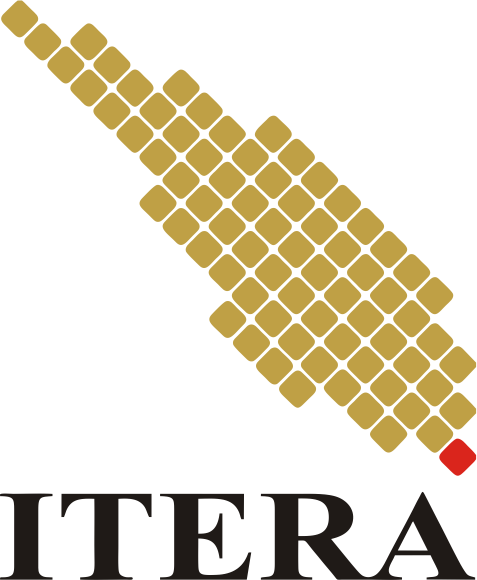
\includegraphics[width=2.1cm, height=2.5cm, keepaspectratio]{figures/itera-logo}
    \end{figure}

	\large \bfseries \MakeUppercase{\thetitle}
	\vfill

    \large \uppercase{TUGAS AKHIR}
    \vfill

    \normalsize \normalfont \theauthor\\
    \printnim
    \vfill

    \normalsize \bfseries
    \uppercase{
        Program Studi Sains Data \\
        Fakultas Sains\\
        Institut Teknologi Sumatera\\
        Lampung Selatan
    }\medskip

    %\thedate
    % automatic year
    \the\year{}

\end{center}

\clearpage
 % Hardcover
%\clearpage
\pagestyle{empty}
\phantomsection% 
\addcontentsline{toc}{chapter}{Halaman Judul}

\begin{center}
\smallskip

    \begin{figure}[h]
    	\centering
    	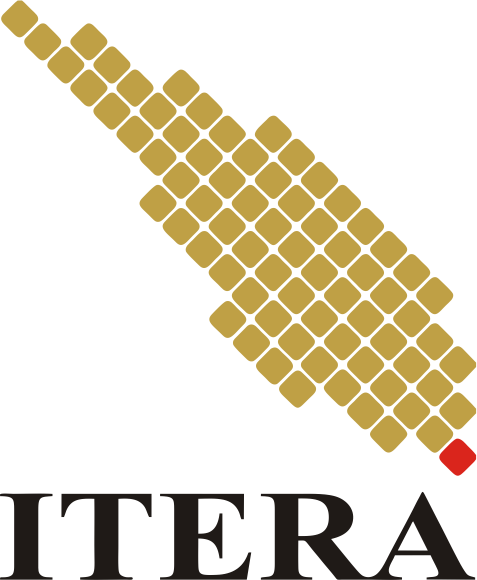
\includegraphics[width=2.1cm, height=2.5cm, keepaspectratio]{figures/itera-logo}
    \end{figure}

	\large \bfseries \MakeUppercase{\thetitle}
	\vfill

    \large \uppercase{Tugas Akhir}\\
    {\normalsize \normalfont Diajukan sebagai syarat untuk memperoleh gelar sarjana}
    \vfill

    \normalsize \normalfont \theauthor\\
    \printnim
    \vfill

    \normalsize \bfseries
    \uppercase{
        Program Studi Sains Data \\
        Fakultas Sains\\
        Institut Teknologi Sumatera\\
        Lampung Selatan
    }\medskip

    %\thedate
    % automatic year
    \the\year{}

\end{center}

\clearpage
 % Softcover
\clearpage
\pagestyle{fancy}
\fancyhf{}
\fancyhead[R]{\thepage}
\phantomsection% 
\addcontentsline{toc}{chapter}{LEMBAR PENGESAHAN}

\begin{center}

%	\chapter*{\normalsize{Lembar Pengesahan}}
	\large \bfseries \MakeUppercase{Lembar Pengesahan} \linebreak
    
    \normalsize \normalfont \onehalfspacing \justify{
    Tugas Akhir Sarjana dengan judul \textbf{\thetitle} \ adalah benar dibuat oleh saya sendiri dan belum pernah dibuat dan diserahkan sebelumnya, baik sebagian ataupun seluruhnya, baik oleh saya ataupun orang lain, baik di Institut Teknologi Sumatera maupun di institusi pendidikan lainnya.}

	Lampung Selatan, \today{} % TODO: automatic date

	\setlength{\tabcolsep}{0pt}
%	\begin{tabular}{l@{\hskip 0.5in}r}
	\begin{tabular}{p{0.7\textwidth}p{0.3\textwidth}}
		Penulis, & \multirow{6}{*}{
			% Kotak pasfoto 3x4
			\begin{tikzpicture}
				\draw rectangle (3cm,4cm) node[pos=.5]{
					{\begin{tabular}{l}
					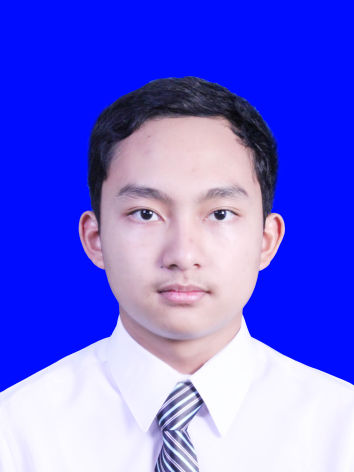
\includegraphics[width=.23\textwidth]{figures/pasfoto.jpg}
					\end{tabular}}};
			\end{tikzpicture}
			}\\
		& \\
		& \\
		& \\
		& \\
		\theauthor\\
		NIM \printnim
	\end{tabular}
	\vfill

	\centering Diperiksa dan disetujui oleh,
	\vspace{2em} % add space
	\justify
    \setlength{\tabcolsep}{0pt}
    \begin{tabular}{p{0.5\textwidth}p{0.5\textwidth}}
        \multicolumn{1}{c}{Pembimbing I,} & \multicolumn{1}{c}{Pembimbing II,} \\
        & \\
        & \\
        & \\
        & \\
		\multicolumn{1}{c}{\underline{\printnamadosbinga}} & \multicolumn{1}{c}{\underline{\printnamadosbingb}} \\
		\multicolumn{1}{c}{\printnipdosbinga} & \multicolumn{1}{c}{\printnipdosbingb} \\
    \end{tabular}
	\vfill

	\centering 
	\begin{tabular}{c}
		Disahkan oleh,\\
		Koordinator Program Studi Sains Data\\
		Fakultas Sains\\
		Institut Teknologi Sumatera
		\\
		\\
		\\
		\\
		\\
		\underline{Tirta Setiawan, S.Pd., M.Si.} \\ % TODO: make automatic
		NIP 199008222022031003 \\
	\end{tabular}
	
\end{center}
\clearpage

%\clearpage
\phantomsection% 
\addcontentsline{toc}{chapter}{Halaman Pernyataan Orisinalitas}

\begin{center}
	\smallskip
	
%	\chapter*{\normalsize{Halaman Pernyataan Orisinalitas}}
	\normalsize \bfseries \MakeUppercase{Halaman Pernyataan Orisinalitas} \linebreak
	
	\normalsize \onehalfspacing{
		Tugas Akhir ini adalah karya saya sendiri, dan semua sumber baik yang dikutip maupun dirujuk telah saya nyatakan benar}
	\vspace{3cm}
	
	\centering 
	\begin{tabular}{l l}
		Nama 			& : \theauthor \\
		& \\
		NIM 			& : \printnim \\
		& \\
		Tanda Tangan 	& : ................................... \\
		& \\
		Tanggal 		& : ................................... \\
	\end{tabular}
	
\end{center}
\clearpage

%\clearpage
\phantomsection% 
\addcontentsline{toc}{chapter}{Halaman Persetujuan Publikasi}

\begin{center}
	\smallskip
	
	\normalsize \bfseries \MakeUppercase{
		HALAMAN PERNYATAAN PERSETUJUAN PUBLIKASI \\
		TUGAS AKHIR UNTUK KEPENTINGAN AKADEMIS
	}\linebreak
	
	\normalsize \normalfont \onehalfspacing \justifying{
		Sebagai civitas akademik Institut Teknologi Sumatera, saya yang bertanda tangan di bawah ini:}
	
	\flushleft
	\setlength{\tabcolsep}{0pt}
	\begin{tabular}{l l}
		Nama 			&  : \theauthor\\
		NIM 			&  : \printnim\\
		Program Studi \	&  : Sains Data\\
		Jurusan 		&  : Fakultas Sains\\
		Jenis Karya 	&  : Tugas Akhir\\
	\end{tabular}

	\justifying
	demi pengembangan ilmu pengetahuan, menyetujui untuk memberikan kepada Institut Teknologi Sumatera \textbf{Hak Bebas Royalti Noneksklusif (Non-exclusive Royalty Free Right)} atas karya ilmiah saya yang berjudul: 
	
	\centering
	\textbf{\thetitle}
	
	\justifying
	beserta perangkat yang ada (jika diperlukan). Dengan Hak Bebas Royalti Noneksklusif ini Institut Teknologi Sumatera berhak menyimpan, mengalihmedia/formatkan, mengelola dalam bentuk pangkalan data (database), merawat, dan memublikasikan tugas akhir saya selama tetap mencantumkan nama saya sebagai penulis/pencipta dan sebagai pemilik Hak Cipta.
	
	Demikian pernyataan ini saya buat dengan sebenarnya. \\
	
	\centering
	Dibuat di : Lampung Selatan\\
	Pada tanggal : \today{}\\ % Automatic date
	\vspace{3cm}
	Yang menyatakan (\theauthor)
	
	
\end{center}
\clearpage

%
%\clearpage

\singlespacing{
	\textbf{\thetitle}\\
	\mbox{\theauthor \ (\printnim)}\\
	Pembimbing I \printnamadosbinga\\
	Pembimbing II \printnamadosbingb\\
}

%\chapter*{ABSTRAK}
\normalsize \bfseries \centering \MakeUppercase{Abstrak}
\phantomsection% 
\addcontentsline{toc}{chapter}{Abstrak}
\\[2\baselineskip]

%taruh abstrak bahasa indonesia di sini
\justifying \normalfont \normalsize{

}

\textbf{Kata Kunci}: Kata Kunci 1, Kata Kunci 2
\clearpage
%\clearpage

\begin{minipage}{\textwidth}
	\singlespacing{
	\textbf{\thetitleEN}\\
	\mbox{\theauthor \ (\printnim)}\\
	Pembimbing I \printnamadosbinga\\
	Pembimbing II \printnamadosbingb\\
}
\end{minipage}

%\chapter*{ABSTRAK}
\normalsize \bfseries \centering \MakeUppercase{Abstract}
\phantomsection% 
\addcontentsline{toc}{chapter}{Abstract}
\\[2\baselineskip]

%taruh abstrak bahasa inggris di sini
\justifying \normalfont \normalsize{

}

\textbf{Keyword}: Keyword 1, Keyword 2
\clearpage
%\clearpage

\normalsize \bfseries \centering \MakeUppercase{Motto}
\phantomsection% 
\addcontentsline{toc}{chapter}{Motto}
\\[2\baselineskip]

\justifying \normalfont{
	% Motto

}

\clearpage
%\clearpage

% PS: Ada bug dimana jika menge-build dari file ini, ada error. Tapi halamannya
% sendiri tidak error jika dibuild dari file lain. (Radhinka)

\normalsize \bfseries \centering \MakeUppercase{Persembahan}
\phantomsection% 
\addcontentsline{toc}{chapter}{Persembahan}
\\[2\baselineskip]

\justifying \normalfont{
	% Kata-kata persembahan
	\blindtext
}

\clearpage
%\clearpage

\normalsize \bfseries \centering \MakeUppercase{Kata Pengantar}
\phantomsection% 
\addcontentsline{toc}{chapter}{Kata Pengantar}
\thispagestyle{fancy}
\fancyhf{}
\fancyhead[R]{\thepage}
\\[2\baselineskip]

\normalsize \normalfont \justifying
(Tuliskan maksud penulisan laporan, misal “Laporan penelitian ini dimaksud kan untuk memenuhi salah ”.........Pada halaman ini mahasiswa berkesempatan untuk menyatakan terima kasih secara tertulis kepada pembimbing dan pihak lain yang telah memberi bimbingan, nasihat, saran dan kritik, kepada mereka yang telah membantu melakukan penelitian, kepada perorangan atau lembaga yang telah memberi bantuan keuangan, materi dan/atau sarana.

Cara menulis kata pengantar beraneka ragam, tetapi hendaknya menggunakan kalimat yang baku. Ucapan terima kasih agar dibuat tidak berlebihan dan dibatasi pada pihak yang terkait secara ilmiah (berhubungan dengan subjek/materi penelitian). 

\flushright{
	Tempat penyusunan TA, tgl-bln-thn\\
	Penulis,
	\\[5\baselineskip]
	\theauthor
}

\clearpage


\addcontentsline{toc}{chapter}{DAFTAR ISI}
\tableofcontents
\addcontentsline{toc}{chapter}{DAFTAR GAMBAR}
{%
    \let\oldnumberline\numberline%
    \renewcommand{\numberline}{\figurename~\oldnumberline}%
    \listoffigures%
}
\addcontentsline{toc}{chapter}{DAFTAR TABEL}
{%
    \let\oldnumberline\numberline%
    \renewcommand{\numberline}{\tablename~\oldnumberline}%
    \listoftables%
}


\cleardoublepage

% Index
%\cleardoublepage
%\addcontentsline{toc}{chapter}{\listappendixname}
%\listofappendices

%\clearpage

\chapter*{Daftar Simbol}
\thispagestyle{fancy}
\fancyhf{}
\fancyhead[R]{\thepage}

\justifying
(Tuliskan maksud penulisan laporan, misal “Laporan penelitian ini dimaksud kan untuk memenuhi salah ”.........Pada halaman ini mahasiswa berkesempatan untuk menyatakan terima kasih secara tertulis kepada pembimbing dan pihak lain yang telah memberi bimbingan, nasihat, saran dan kritik, kepada mereka yang telah membantu melakukan penelitian, kepada perorangan atau lembaga yang telah memberi bantuan keuangan, materi dan/atau sarana.

Cara menulis kata pengantar beraneka ragam, tetapi hendaknya menggunakan kalimat yang baku. Ucapan terima kasih agar dibuat tidak berlebihan dan dibatasi pada pihak yang terkait secara ilmiah (berhubungan dengan subjek/materi penelitian). 
